\section{INTRODUÇÃO}\label{sec:intro}
    \subsection{Tema}

\begin{onehalfspacing}
    \begin{justify}
        \begin{large}
            Texto. Texto. Texto. Texto. Texto. Texto. Texto. Texto. Texto. Texto. Texto. Texto. Texto. Texto. Texto. Texto. Texto. Texto. Texto. Texto. Texto. Texto. Texto. Texto. Texto. Texto. Texto. Texto. Texto. Texto. Texto. Texto. Texto. Texto. Texto. Texto. Texto. Texto. Texto. Texto. Texto. Texto. Texto. Texto. Texto. Texto. Texto. Texto. Texto. Texto. Texto. Texto. Texto. Texto. Texto. Texto. Texto. Texto. Texto. Texto. Texto. Texto. Texto. Texto. Texto. Texto. Texto. Texto. Texto. Texto. Texto. Texto. Texto. Texto. Texto. Texto. Texto. Texto. Texto. Texto. Texto. Texto. Texto. Texto. Texto. Texto. Texto. Texto. Texto. Texto. Texto. Texto. Texto. Texto. Texto. Texto. Texto. Texto. Texto. Texto. Texto. Texto. Texto. Texto. Texto. Texto. Texto. Texto. Texto. Texto. Texto. Texto. Texto. Texto. Texto. Texto. Texto. Texto. Texto. Texto. Texto. Texto. Texto. Texto. Texto. Texto. Texto. Texto. Texto. Texto. Texto. Texto. Texto. Texto. Texto. Texto.
        \end{large}
    \end{justify}
\end{onehalfspacing}

\begin{figure}[ht]\caption{Gráfico - Relatório de Vacância}
    \centering
        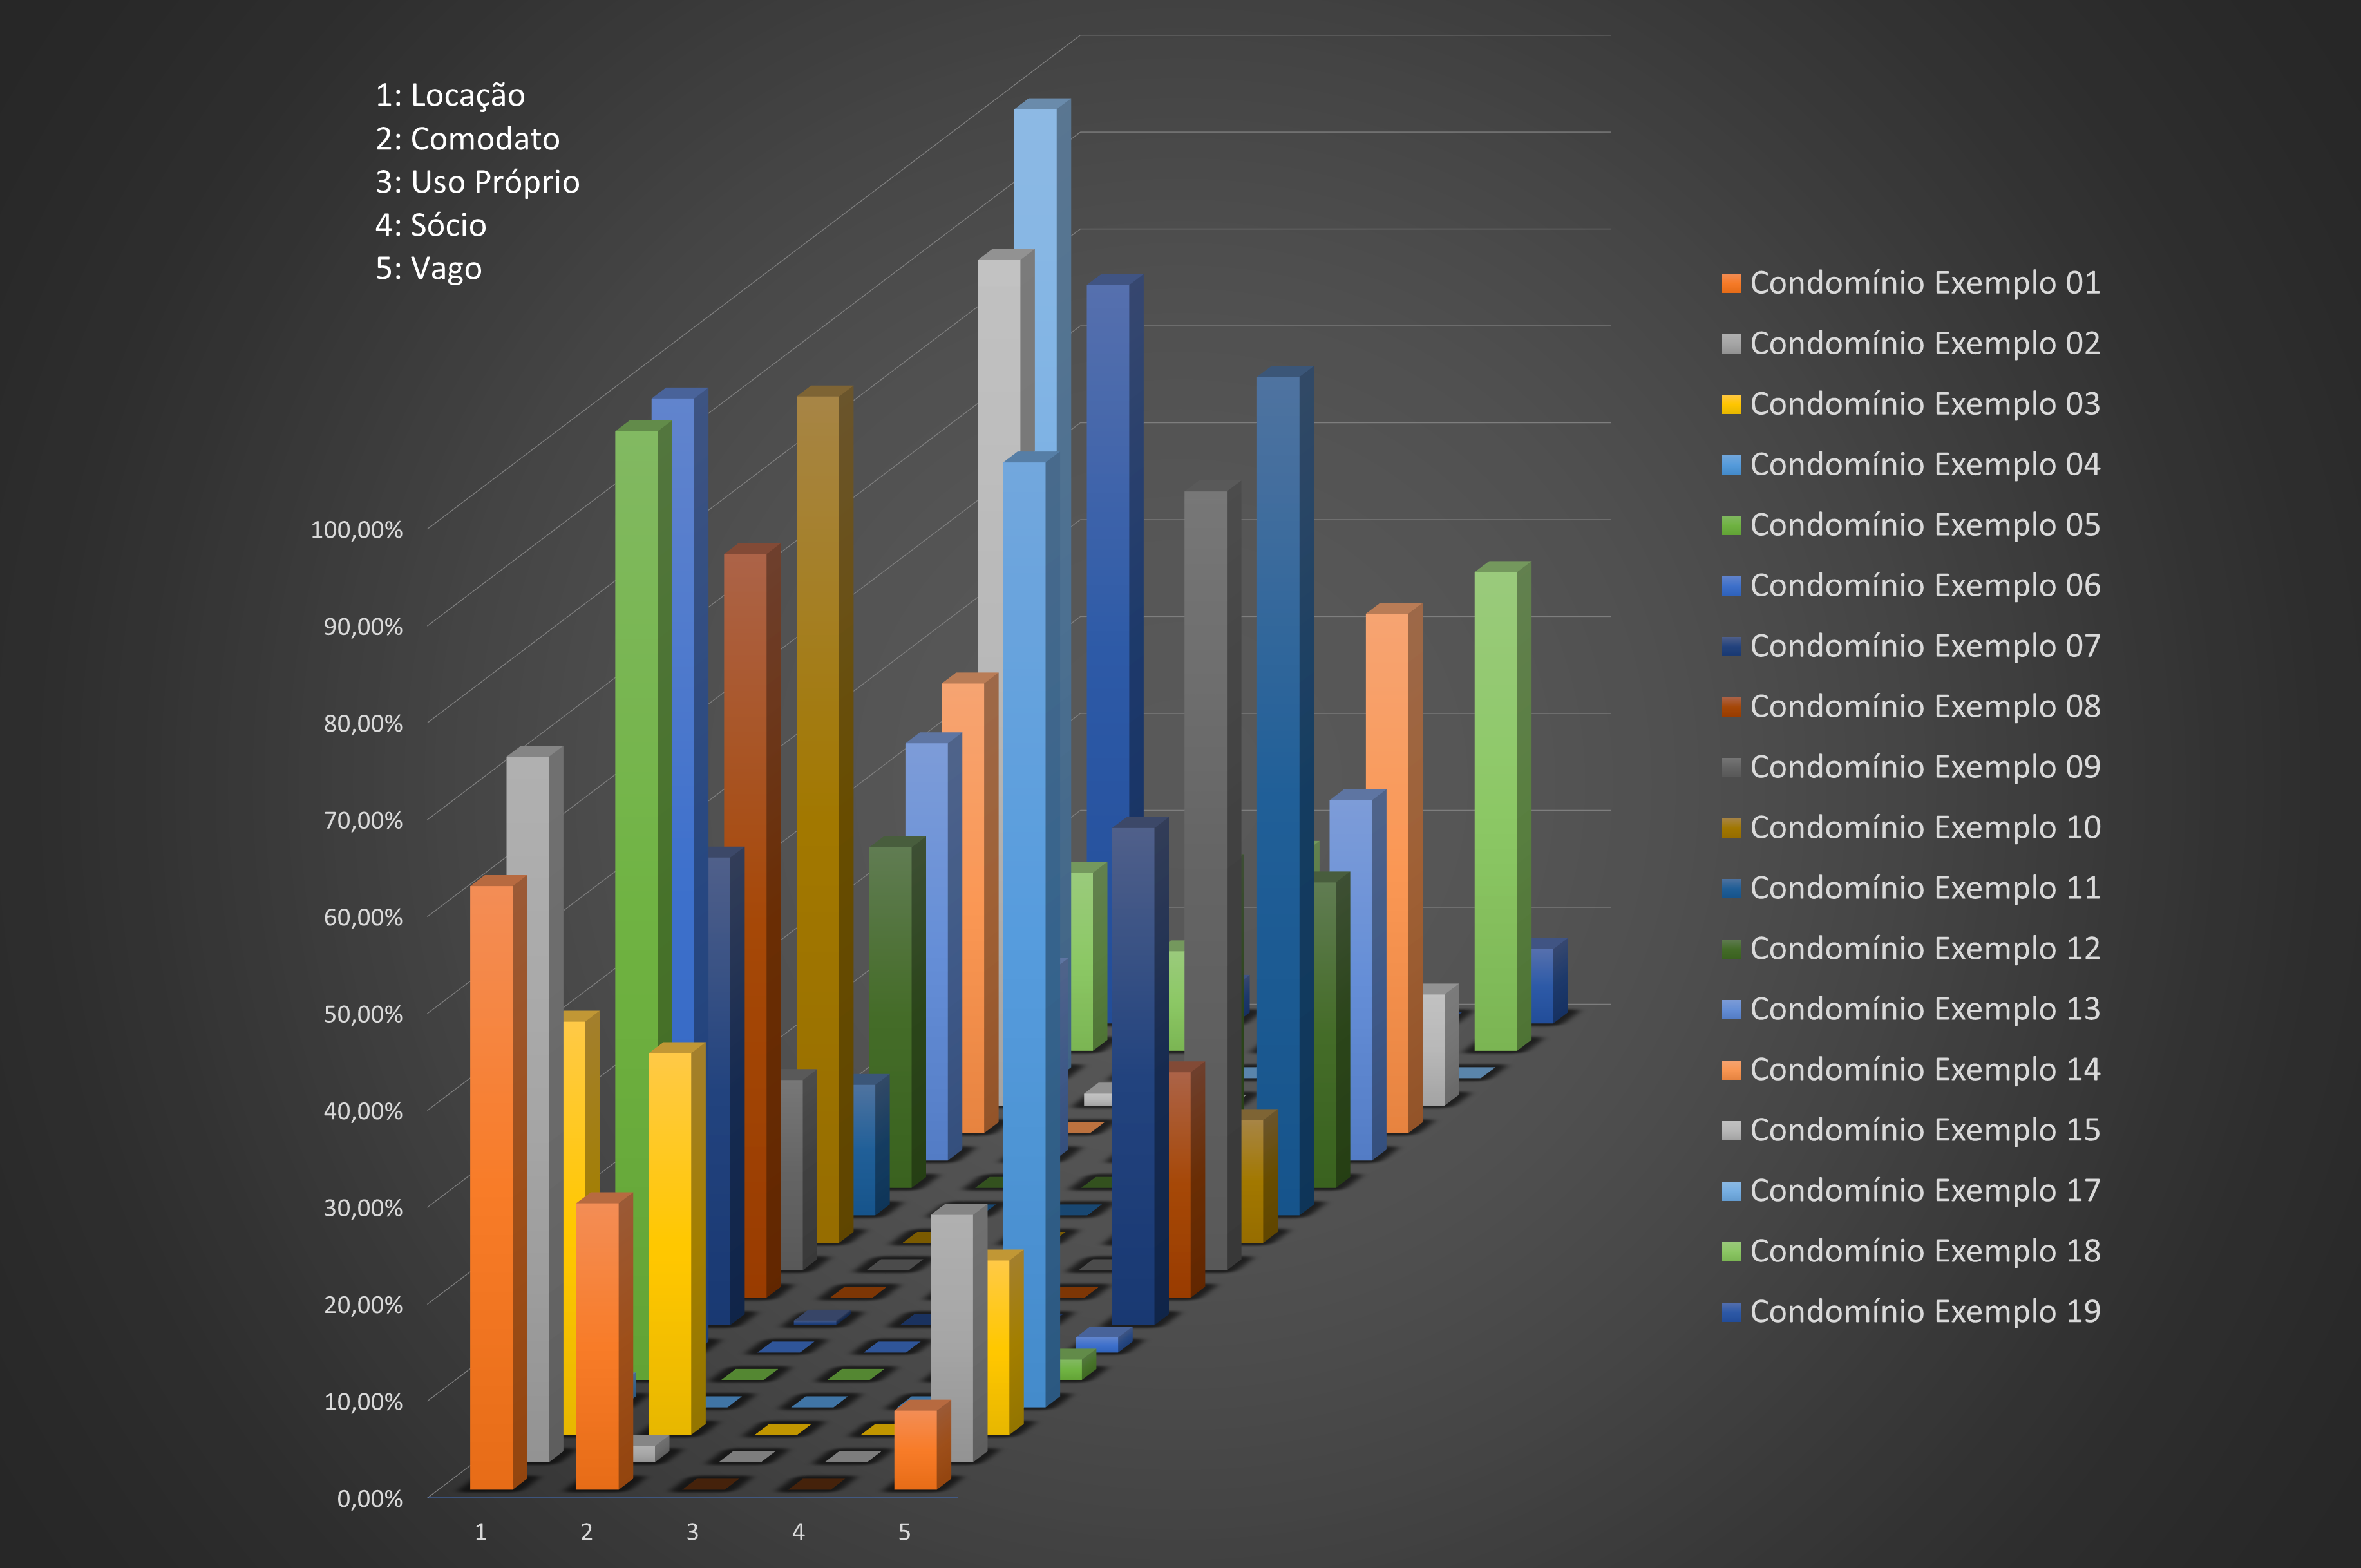
\includegraphics[scale = 0.5]{images/relatorio-vacancia.png}
        \label{figure:tiposdeinovacao}
\end{figure}
\begin{flushleft}
    \begin{small}
        Fonte: adaptado de Vitória Peçanha de Araújo (2021).\\
    \end{small}
\end{flushleft}

\begin{onehalfspacing}
    \begin{justify}
        \begin{large}
            Texto. Texto. Texto. Texto. Texto. Texto. Texto. Texto. Texto. Texto. Texto. Texto. Texto. Texto. Texto. Texto. Texto. Texto. Texto. Texto. Texto. Texto. Texto. Texto. Texto. Texto. Texto. Texto. Texto. Texto. Texto. Texto. Texto. Texto. Texto. Texto. Texto. Texto. Texto. Texto. Texto. Texto. Texto. Texto. Texto. Texto. Texto. Texto. Texto. Texto. Texto. Texto. Texto. Texto. Texto. Texto. Texto. Texto. Texto. Texto. Texto. Texto. Texto. Texto. Texto. Texto. Texto. Texto. Texto. Texto. Texto. Texto. Texto. Texto. Texto. Texto. Texto. Texto. Texto. Texto. Texto. Texto. Texto. Texto. Texto. Texto. Texto. Texto. Texto. Texto. Texto. Texto. Texto. Texto. Texto. Texto. Texto. Texto. Texto. Texto. Texto. Texto. Texto. Texto. Texto. Texto. Texto. Texto. Texto. Texto. Texto. Texto. Texto. Texto. Texto. Texto. Texto. Texto. Texto. Texto. Texto. Texto. Texto. Texto. Texto. Texto. Texto. Texto. Texto. Texto. Texto. Texto. Texto. Texto. Texto.
        \end{large}
    \end{justify}
\end{onehalfspacing}\pagebreak

%----------------> JUSTIFICATIVA <-------------------
    \subsection{Justificativa}
    
\begin{onehalfspacing}
    \begin{justify}
        \begin{large}
            Texto. Texto. Texto. Texto. Texto. Texto. Texto. Texto. Texto. Texto. Texto. Texto. Texto. Texto. Texto. Texto. Texto. Texto. Texto. Texto. Texto. Texto. Texto. Texto. Texto. Texto. Texto. Texto. Texto. Texto. Texto. Texto. Texto. Texto. Texto. Texto. Texto. Texto. Texto. Texto. Texto. Texto. Texto. Texto. Texto. Texto. Texto. Texto. Texto. Texto. Texto. Texto. Texto. Texto. Texto. Texto. Texto. Texto. Texto. Texto. Texto. Texto. Texto. Texto. Texto. Texto. Texto. Texto. Texto. Texto. Texto. Texto. Texto. Texto. Texto. Texto. Texto. Texto. Texto. Texto. Texto. Texto. Texto. Texto. Texto. Texto. Texto. Texto. Texto. Texto. Texto. Texto. Texto. Texto. Texto. Texto. Texto. Texto. Texto. Texto. Texto. Texto. Texto. Texto. Texto. Texto. Texto. Texto. Texto. Texto. Texto. Texto. Texto. Texto. Texto. Texto. Texto. Texto. Texto. Texto. Texto. Texto. Texto. Texto. Texto. Texto. Texto. Texto. Texto. Texto. Texto. Texto. Texto. Texto. Texto.
        \end{large}
    \end{justify}
\end{onehalfspacing}

%------------------> OBJETIVOS <---------------------
    \subsection{Objetivos}

\begin{onehalfspacing}
    \begin{justify}
        \begin{large}
            Texto. Texto. Texto. Texto. Texto. Texto. Texto. Texto. Texto. Texto. Texto. Texto. Texto. Texto. Texto. Texto. Texto. Texto. Texto. Texto. Texto. Texto. Texto. Texto. Texto. Texto. Texto. Texto. Texto. Texto. Texto. Texto. Texto. Texto. Texto. Texto. Texto. Texto. Texto. Texto. Texto. Texto. Texto. Texto. Texto. Texto. Texto. Texto. Texto. Texto. Texto. Texto. Texto. Texto. Texto. Texto. Texto. Texto. Texto. Texto. Texto. Texto. Texto. Texto. Texto. Texto. Texto. Texto. Texto. Texto. Texto. Texto. Texto. Texto. Texto. Texto. Texto. Texto. Texto. Texto. Texto. Texto. Texto. Texto. Texto. Texto.
        \end{large}
    \end{justify}
\end{onehalfspacing}

%------------------> TABELA 1 <---------------------
\begin{onehalfspacing}
    \renewcommand\tabularxcolumn[1]{>{\Centering}m{#1}} 
        \begin{table}[ht]
        \caption{Tabela de exemplo de tema}
            \begin{center}\large
                \begin{tabularx}{\textwidth}{|X|X|}
                    \hline
                    \textbf{Texto 1} \cellcolor{black!20} & \textbf{Texto 2} \cellcolor{black!20}  \\
                    \hline
                    Texto. Texto. Texto. Texto. Texto. Texto. Texto. Texto. Texto. \cellcolor{black!5} & \textbf{Texto 3}
                        
                    Descrição, descrição, descrição
                    
                    \textbf{Texto 4}
                        
                    Descrição - Descrição
                    Descrição - Descrição

                    \textbf{Texto 5}
                        
                    Dados - Dados, dados
                        
                    Dados - Dados, dados

                    \textbf{Texto 6}
                        
                    000×000

                    \textbf{Texto 7}
                        
                    Descrição, descrição, descrição AAAA 1.0 \cellcolor{black!5} \\
                \hline
            \end{tabularx}
        \end{center}
        \begin{small}
            Fonte: adaptado de Autor (2021).\\
        \end{small}
    \end{table}
\end{onehalfspacing}

\begin{onehalfspacing}
    \begin{justify}
        \begin{large}
            Texto. Texto. Texto. Texto. Texto. Texto. Texto. Texto. Texto. Texto. Texto. Texto. Texto. Texto. Texto. Texto. Texto. Texto. Texto. Texto. Texto. Texto. Texto. Texto. Texto. Texto. Texto. Texto. Texto.
        \end{large}
    \end{justify}
\end{onehalfspacing}\pagebreak




